\documentclass[12pt]{report}
\usepackage{common}
\usepackage[round]{natbib}
\usepackage[strings]{underscore}
\usepackage{url}
\usepackage{todonotes}
\usepackage[toc]{appendix}
\usepackage{setspace}
\usepackage{hyperref}
\usepackage[english]{babel}
\usepackage{amsthm}
\usepackage{caption}

\newcommand\numberthis{\addtocounter{equation}{1}\tag{\theequation}}
\newtheorem{theorem}{Theorem}

\pagenumbering{roman}
\title{Document Summarization (draft)}
\author{Jeffrey Ling}
%\date{}
\begin{document}
\maketitle{}
\onehalfspacing

\begin{abstract} % needs work
While humans are naturally able to produce high-level summaries upon reading paragraphs of text, computers still find such a task enormously difficult. Despite progress over the years, the general problem of document summarization remains intractable and 

Inspired by recent work in deep learning, we apply the sequence-to-sequence (seq2seq) model with attention to the summarization problem. While seq2seq models are successful in a variety of natural language processing tasks, the computation does not scale well to tasks with long sequences such as documents. To that end, we propose a novel coarse-to-fine attention method to reduce the computational complexity of the standard attention model.
%By organizing the source sequence into a 2-dimensional image, we hierarchically apply attention, using a coarse mechanism for the first layer to select a row sequence, and a finer mechanism for the second soft attention layer. While the computation for training standard seq2seq models scales linearly with source sequence length, our method is invariant to length and thus can scale arbitrarily.

We evaluate our model on the CNN/Dailymail document summarization dataset. Results...
\end{abstract}

\tableofcontents{}
\pagenumbering{arabic}



\chapter{Introduction}

\section{Natural Language Processing}

The field of natural language processing arises from a very simple question: how can we teach machines to read, speak, and understand the words that we use with such ease and fluency?

Such a question has been considered since the first computers were built. The classic Turing test, posed by Alan Turing in 1950, requires a machine to converse in a way that is indistinguishable from a human, and thus requires a fundamental grasp on how to properly use language.
Although it was simple for Turing to conceptualize what a successful machine might look like, many have been stumped on how to actually construct such a system.
Indeed, to this day, no machine has been able to fully pass the Turing test as it was originally posed.


While computers can now run computations at a rate that far exceeds human cognition, language tasks that we consider trivial still prove to be extraordinarily difficult for a machine to solve. Consider the problem of deciding words with multiple meanings such as ``bass'' (word sense disambiguation), or the problem of identifying to what or whom a certain pronoun refers (coreference). 
While humans reliably perform these functions on a daily basis, they are not at all easy for computers to handle.


However, the need for computers to understand language has never been greater.
In today's information age, NLP grows increasingly important as the accumulation of free-form text begins to outpace the ability of humans to process it. In fields such as medicine, this can mean missed diagnoses; in law, wasted effort on irrelevant documents; in international relations, misinterpretations of foreign articles.
Because natural language is everywhere and used by everyone, the demand for text processing solutions remains as high as ever.

\section{Methods in NLP}

We have established that NLP is a difficult yet worthwhile undertaking. In this section, we investigate the general philosophy of tackling these hard problems.

The key property of language that make it difficult for machines to handle is its discrete and combinatorial nature. When we form sentences, we can string together arbitrary words from our vocabulary, as long as we follow the rules of some highly structured grammar. In some sense, the essential difficulty in NLP lies in handling these complicated structured problems.

Linguistics attempts to answer this by building a formal theory of language. Indeed, many ideas from linguistics, including sentence parses, morphology, and semantics are invaluable in NLP for understanding the rules for how sentences and phrases can be put together.
In order to solve a language problem, we might begin by enriching the surface form of text (the raw sentences and paragraphs) with the parse structure, parts of speech, coreferent entities, etc. We can then use this featurized form of language in whichever way we prefer.

\begin{figure}[t]
\centering
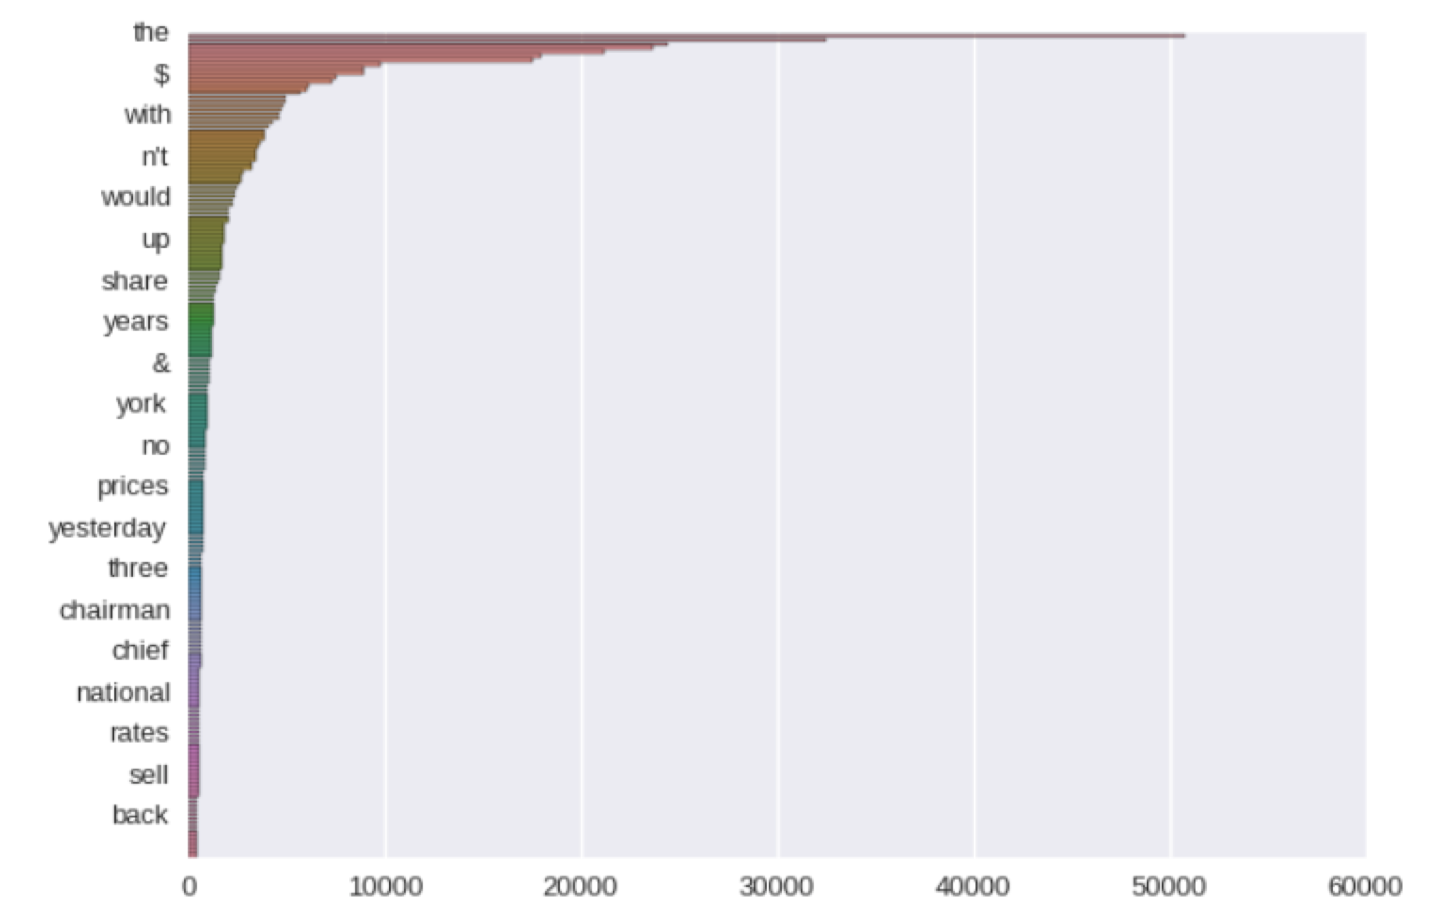
\includegraphics[scale=0.5]{images/zipf}
\caption{Zipf's law, indicating the relationship between English words and their frequency. The distribution approximately follows an inverse power law. Image from CS287}
\label{fig:zipf}
\end{figure}

Another mode of thought focuses on the role of statistics in language. A cursory examination of the distribution of English words reveals an interesting power law distribution known as Zipf's law (figure~\ref{fig:zipf}). By drawing from ideas of information theory \citep{Shannon1948}, we can treat language as the result of some noisy probabilistic process, and we can reduce problems such as language modeling to learning parameters of some simple distributions.

Historically, there has been contention about the roles of linguistics and statistics in NLP. Certain practical problems seem to be better off without linguistic theory; as IBM researcher Frederick Jelinek famously said, ``Every time I fire a linguist, the performance of the speech recognizer goes up.'' \todo{citation} Indeed, even naive models of language seem to perform well if given enough training data, as evidenced by the IBM models for machine translation \citep{Brown1993}.

Today, the linguistics-free approach has been taken to an extreme by deep learning systems. For the first time, neural networks are able to learn to perform language tasks in an end-to-end fashion \citep{Collobert2011}, i.e. without the linguistic preprocessing that was once considered necessary.
Neural methods have been adopted by user-facing systems like Google Translate with great success \citep{GoogleTranslate2016}.


\section{Automatic Summarization}
\label{sec:taxonomy}

In this thesis, we will consider the particular problem of \emph{text summarization}. That is, given a document with several sentences of text, the goal is to produce a short summary that captures most or all of its salient points.


\citet{Nenkova2011} give a comprehensive overview of the problem of summarization. In particular, they provide a taxonomy of methods that researchers have developed to tackle the task:

\paragraph{Extractive vs. abstractive} Extractive summaries extract certain sentences or phrases from the document, while abstractive summaries take a more holistic view and can in practice be anything (similar to how humans produce summaries). 

Extractive methods are by far more popular due to the simplicity of building an extraction algorithm. Abstractive methods is much more difficult, as not only do we need to extract relevant content, but we also need to ensure grammaticality of the output (a difficult problem in itself).

\paragraph{Single- vs. multi-document} Summarization was originally posed as the problem of producing a summary for a single document. However, with the onset of the Internet, there are often multiple documents on the same topic, and so a summarization system should be able to use all of them to produce a summary.

Interestingly, it has been noted that the multi-document problem is often easier due to redundant information across sources.

%\paragraph{Indicative (style) vs. informative (facts)} Indicative summaries provide a sense for what a certain document is about without necessarily giving all of its details, while informative summaries are meant to replace the original document in terms of content.

\paragraph{Keyword vs. headline} Keyword summaries are allowed to simply be a bag-of-words of important keywords from the document, while headline summaries must form a coherent sentence.

\paragraph{Generic vs. query-focused} Generic summaries make no assumptions about the reader and are meant to be generally informative, while query-focused summaries take into consideration a query and only return relevant information.

The contrast between these two methods highlights an important question in summarization: to what end are we summarizing documents? If we can answer this question, we can build systems to more accurately accomplish our desired tasks.

\vspace{0.5cm}


Most of this taxonomy is based upon insights from DUC (Document Understanding Conferences), a set of tasks released by NIST between 2001-2006 to promote research in summarization \citep{over2007duc}.

The DUC tasks were fairly diverse and varied from year to year. DUC 2001 and 2002 asked for generic summaries of news articles, while DUC 2003 presented a multi-document problem. DUC 2004-2006 shifted to a more question-answering based approach, and many of the documents were accompanied by focused queries.

While DUC did not lead to any definitive answers on how best to summarize documents, some important empirical discoveries were noted.
For the generic summarization tasks, it was found that the first sentence of news articles was a strong baseline that more sophisticated methods found hard to beat. Thus, the generic summary task was seen as ill-formed and not as interesting, leading to the more query-focused tasks in the later years.


DUC also inspired a lot of thinking on the best way to evaluate summaries. Evaluating a good summary is inherently ambiguous, and probably one of the hardest parts of the problem. While a single most effective metric for summarization may not exist, DUC established several important criteria, including grammaticality, non-redundancy, and content coverage.


For extractive summaries, people have proposed simple metrics such as precision and recall on selected sentences. These naturally do not work too well since 1) not all sentences are equally informative, and 2) not all parts of a sentence are relevant.

When we don't have sentence labels as in the extractive case, evaluation is harder. One proposed metric is recall on elementary discourse units (EDUs), labeled clauses within a summary that ought to be captured. ROUGE \citep{lin2004rouge}, inspired by the BLEU metric for machine translation \citep{Papineni2002}, is a cheap and fast method based on n-gram precision, recall, and length considerations.


None of these methods directly address the grammaticality of the output. Aside from using human evaluation, meaningful metrics for summaries is still very much an open question \citep{toutanova2016summarymetrics}.


\vspace{0.5cm}

 

%It is important to highlight these differences to understand how people thought about the problem. The complexity of this taxonomy indicates that the summarization problem in its simplest formulation is very poorly defined. Indeed, query-focused summarization may well be a useful task, but it may be more accurate to classify it as question-answering rather than summarization.


Going forward, we will limit our scope to the single-document, headline, and generic summarization case. We will explore a few different algorithms in extractive and abstractive summarization, and connect these approaches with recent trends in deep learning.

\section{Summarization Methods}

One of the first treatises on automatically producing summaries was \citet{luhn1958automatic}, which considered the problem of producing abstracts for scientific articles. At the time, computers were still monolithic machines that ran on punch cards, so automating the summarization process was quite ahead of its time.

\citet{luhn1958automatic} proposed a simple sentence-ranking method to produce summaries. The algorithm gives each sentence a score based on the occurrence of frequently appearing words. This is one of the first examples of an extractive summarization method.

Since then, a variety of approaches have been used to solve summarization. We highlight some notable work in both the extractive and abstractive frameworks.

\subsection{Extractive} The most popular methods for document summarization have generally been extractive due to their simplicity.

There are two natural procedures for extractive summarization: one is to produce a ranking of sentences based on some scoring function, and two is to classify sentences as either in the summary or not. \citet{luhn1958automatic} is an example of the first approach.

\citet{Carbonell1998} extend on the scoring-ranking method with an information metric, MMR (maximum marginal relevance), that penalizes pairwise similarity between sentences. Their work is one of the first that attempt to reduce redundancy in the summary.

\citet{Kupiec1995} pioneer the second method by treating sentence selection as a classification problem. They obtain a training corpus and apply a naive Bayes approach to classify sentences.

Ranking and classifying algorithms became more sophisticated over time, and most of these methods were soon applied to extractive summarization.

\citet{Shen2004} models sentence extraction as a sequential classification problem, training a linear-chain conditional random field to find the best subset of sentences.

 
\citet{svore2007} use a basic neural network as a sentence classifier.


Deep learning models have also been used to extract sentences.

\citet{Cao2015} use convolutional neural networks to extract features for each sentence, combining these with document-level features to produce scores.

\citet{Cheng2016} apply the encoder-decoder model using recurrent neural networks to produce labels for each sentence.

\todo{finish}


\subsection{Abstractive} While extraction has proven to be successful, the method is inherently limited in its ability to summarize. The more challenging method, and also the closest to what humans do, is \emph{abstractive} summarization. Instead of strictly requiring that all words of the summary come from the source document, any coherent text is allowed.

Two methods used to produce abstractive summaries are sentence compression and sentence fusion. Compression removes less useful information from sentences, while fusion is harder and combines information from sentences. % cite Barzilay, MCkeown

Compression: \citet{knight2002summarization} employs a noisy channel model, similar to machine translation, to deduce the ``most probable'' compression, while \citet{clarke2008global} uses an integer linear program. \citet{cohn2008sentence} extend the tree-based methods to allow for insertions and substitutions during compression, whereas prior methods were purely deletion based. \cite{zajic2004topiary} successfully use a sentence compression algorithm along with an unsupervised topic model on the DUC 2004 task.

Fusion: align parse trees and combine phrases that are similar \todo{finish}

\citet{Durrett2016} apply an ILP approach, where they maximize a score based on textual and coreferent features with certain grammaticality and anaphora constraints.


Deep learning has also been successfully applied to abstractive summarization. \citet{rush2015neural} propose a completely data-driven model for headline generation by training an end-to-end model. More recently, \citet{nallapati2016seq2seq} apply the same approach on full documents.

As with deep learning methods for extraction, these models require a large amount of supervised training data. One advantage of the abstractive model is that data in the document-abstract format is more easily obtainable than labeled extractive data.


\subsection{In the Wild}

Outside of the academic realm, summarization is an important problem in industry. One noteworthy summarization method is on Reddit\footnote{\url{reddit.com}}: in order to summarize long forum discussions, Reddit uses technology from Smmry\footnote{\url{smmry.com}}.

Smmry's algorithm is a simple extractive method. It counts word occurrences, splits discussions by sentence, and ranks the sentences based on the sum of their word scores. This algorithm bears extraordinary similarity to \citet{luhn1958automatic} --- although a variety of work has been done since then, the simplest approaches turn out to be the most practical.

\section{Outline}

Inspired by advances in deep learning for NLP, we set out to build a deep model to abstractively generate summaries. Along the way, we propose a new model architecture that extends the sequence-to-sequence model that attempts to reduce the computational complexity of the document summarization problem.


We provide an outline for the rest of this thesis.
In Chapter~\ref{chap:related}, we give a survey of deep learning and motivate its use in solving our problem.
In Chapter~\ref{chap:background}, we provide the necessary background material for understanding our models and algorithms.
In Chapter~\ref{chap:models}, we describe our models formally.
In Chapter~\ref{chap:experiments}, we describe the experimental setup, including our dataset, baselines, and practical details for training our models.
In Chapter~\ref{chap:results}, we show results and analyze the outputs of our models.
Finally, we conclude in Chapter~\ref{chap:conclusion}.

%%%%%%%%%%

\chapter{Related Work}
\label{chap:related}


\section{Deep Learning}

The history of neural networks dates back to the perceptron \citep{Rosenblatt1958}, a simple model that assumes data can be linearly separated. Due to this strict requirement, the machine learning community dismissed the idea as impractical, and research was sidelined for most of the 20th century.

Some other work continued: \citet{Rumelhart1986} showed that the backpropagation algorithm could be used to efficiently train general neural networks, but this was before the era of GPUs and modern computing, and so the algorithm could not be practically used.

Recently, neural networks have made a resurgence. In the ImageNet image classification competition in 2012, \citet{Krizhevsky2012} won using deep convolutional neural networks \citep{LeCun1995}, beating the competition by a significant margin. This led to a renewed wave of research, especially due to the advancement of modern computing power and GPUs, which can train networks at 10 to 20 times the speed of standard CPUs. Today, deep models are successfully used in image recognition \citep{Farabet2013}, speech recognition \citep{Hinton2012}, and Go playing \citep{Silver2016}, just to name a few.

\begin{figure}
\centering
\includegraphics[width=\textwidth]{images/graph}
\caption{A visualization of word2vec word embeddings clusters \citep{mikolov2013word2vec}, projected to two dimensional space (how?). Words with similar semantic meaning tend to be close together in the space. Image from CS287.}
\label{fig:word2vec}
\end{figure}

While neural networks are often treated as black box classifiers, \citet{Zeiler2014} show that the intermediate layers of deep convolutional networks contain abstracted qualities of the input, such as patterns, textures, and objects of the input. This suggests that neural networks are discovering features of the input and building generalized \emph{representations} of their inputs.

The idea of learning representations of the input is quite general, and so it comes as no surprise that deep networks soon found applications in NLP. \citet{mikolov2013word2vec} show that by training a neural network on a Google News text corpus, the network learned to map words in the English language to a vector of real numbers known as \emph{word embeddings}. These word embeddings are actually able to capture semantic properties of the words --- for example, taking the vectors for \emph{king}, \emph{man}, and \emph{woman}, we find that $v_{king} - v_{man} + v_{woman} \approx v_{queen}$, preserving the analogy that we usually make with text.

% diagram of vectors

Since the onset of deep learning, deep models have found their way into nearly every corner of NLP. Much of their success relies on the ubiquity of the \emph{long short-term memory} (LSTM) recurrent neural network \citep{hochreiter1997long}, a model used to both process and generate sequences of text.
Several state-of-the-art algorithms are now based upon deep learning tools such as word vectors and LSTMs. While there is too much to cover here, \citet{goldberg2015primer} provides a concise summary of the models that have had the greatest impact on NLP. % weak



%\section{Summary}
%
%We consider some recent work done in deep neural summarization.
%
%We can frame summarization as a supervised headline generation problem. That is, given a document (the source sequence of words), we desire to produce a shorter headline or summary (the target sequence). 
%
%
%Existing methods in deep learning have proven to be highly effective for this kind of task, especially the sequence-to-sequence (seq2seq) model \citep{sutskever2014sequence, bahdanau2014neural}. 
%
%\citet{rush2015neural} use the seq2seq model to summarize single sentences into headlines, but we consider the more general problem of summarizing arbitrarily long documents.
%
%More recently, seq2seq models have been applied to train both extractive \citep{} and abstractive \citet{nallapati2016seq2seq} summarization systems at the document level. While such work demonstrates the feasibility of deep learning in this problem, it is very preliminary and leaves much room to explore alternative architectures.




\section{Motivation}


Why deep models? There are currently two general approaches to solving problems in NLP: one is to use as much linguistic theory as possible to reduce the problem, and another is to apply black box learners such as deep neural networks.

Deep models work fantastically well on many tasks, especially when it comes to lowering metrics. However, as big of a hammer as deep learning is, there must be nails available for the tool to hit.
In order to further language understanding, datasets and tasks must be posed such that deep models can be applied; it is exactly in this domain that classical theory is still relevant.
As \citet{Manning2016} argues, although neural models have come to dominate NLP papers, there will always be a need for domain experts to prepare the field so that deep learning can succeed.

%On one hand, systems with handcrafted features can perform extremely well if domain specific knowledge can be built in.
%On the other hand, a purely data-driven system can automatically create most of the necessary features, and empirically are proven to work very well.

With this caveat, there are many worthwhile reasons to study deep networks in NLP. First, they work! In fact, they work remarkably well without any feature engineering, which tends to be one of the fussiest parts of building machine learning algorithms.

Second, they are not mutually exclusive with standard feature extraction methods, and so can augment classical methods.

Third, we find that trained models can discover latent structure in language automatically, which may reveal insights about how language is used. As an example, sequence-to-sequence models with attention \citep{bahdanau2014neural} learn the concept of a word alignment in translation without any direct supervision.


It is this third point upon which we base this thesis. Although they began as black-box optimizers, end-to-end deep models are slowly being dissected into more understandable parts. Our goal is to test the hypothesis that such parts are in fact interpretable and are functioning as we expect them to.

With this goal in mind, we attempt to interpretably extend the attention mechanism of existing sequence-to-sequence models, and we analyze its performance on the task of document summarization. In the next chapter, we provide the background for how we will do this.


\todo{needs work} 

%%%%%%%
\chapter{Background}
\label{chap:background}

In this chapter, we set up the relevant background ideas for our models.

\section{Sequence-to-Sequence Attention Models}

Many NLP problems can be posed as follows: given an input sequence of tokens $x_1, \ldots, x_n \in \mcV$, we train a model to produce an output sequence $y_1, \ldots, y_m \in \mcY$. We normally pose this as a probabilistic problem and model the conditional probabilities, so that we wish to find
\begin{equation}
\begin{split}
&\argmax_{y_1, \ldots, y_n \in \mcY} p(y_1, \ldots, y_m | x_1, \ldots, x_n) \\
= & \argmax_{y_1, \ldots, y_n} p(y_1 | x_1, \ldots, x_n)p(y_2 | y_1, x_1, \ldots, x_n) \cdots p(y_m | y_1, \ldots, y_{m-1}, x_1, \ldots, x_n)
\end{split}
\end{equation}

The sequence-to-sequence architecture \citep{sutskever2014sequence}, also known as the encoder-decoder architecture, neatly provides a solution to this framework. By encoding the input $x_1, \ldots, x_n$ into a fixed size vector which we call the \emph{context vector}, we can compute the conditional probabilities and hence generate $y_1, \ldots, y_m$ conditioned on this context vector.

The model has been used to great effect in a variety of NLP tasks, including machine translation \citep{sutskever2014sequence, bahdanau2014neural}, question answering \citep{Hermann2015}, dialogue \citep{li2016persona}, caption generation \citep{xu2015captioning}, and in particular summarization \citep{rush2015neural}.


A popular variant of sequence-to-sequence models are \emph{attention} models \citep{bahdanau2014neural}. The key idea is to keep an encoded representation of all parts of the input, attending to the relevant part each time we produce an output from the decoder. If we have a representation $\boldh_i \in \reals^d$ for input token $x_i$, we model this attention process by computing weights $\alpha_1, \ldots, \alpha_n$ such that $\sum_{i=1}^n \alpha_i = 1$. The resulting context vector is then the weighted average $\sum_{i=1}^n \alpha_i \boldh_i$.

\citet{xu2015captioning} show how attention models can be used to ``summarize'' an image and produce a caption. 
By analyzing where in the image their models attend to when generating each word of the caption, i.e. where $\alpha_i$ is highest in the image, they qualitatively find that the model is essentially describing an object of the image. 
Figure~\ref{fig:caption} shows some examples.

\begin{figure}[t]
\centering
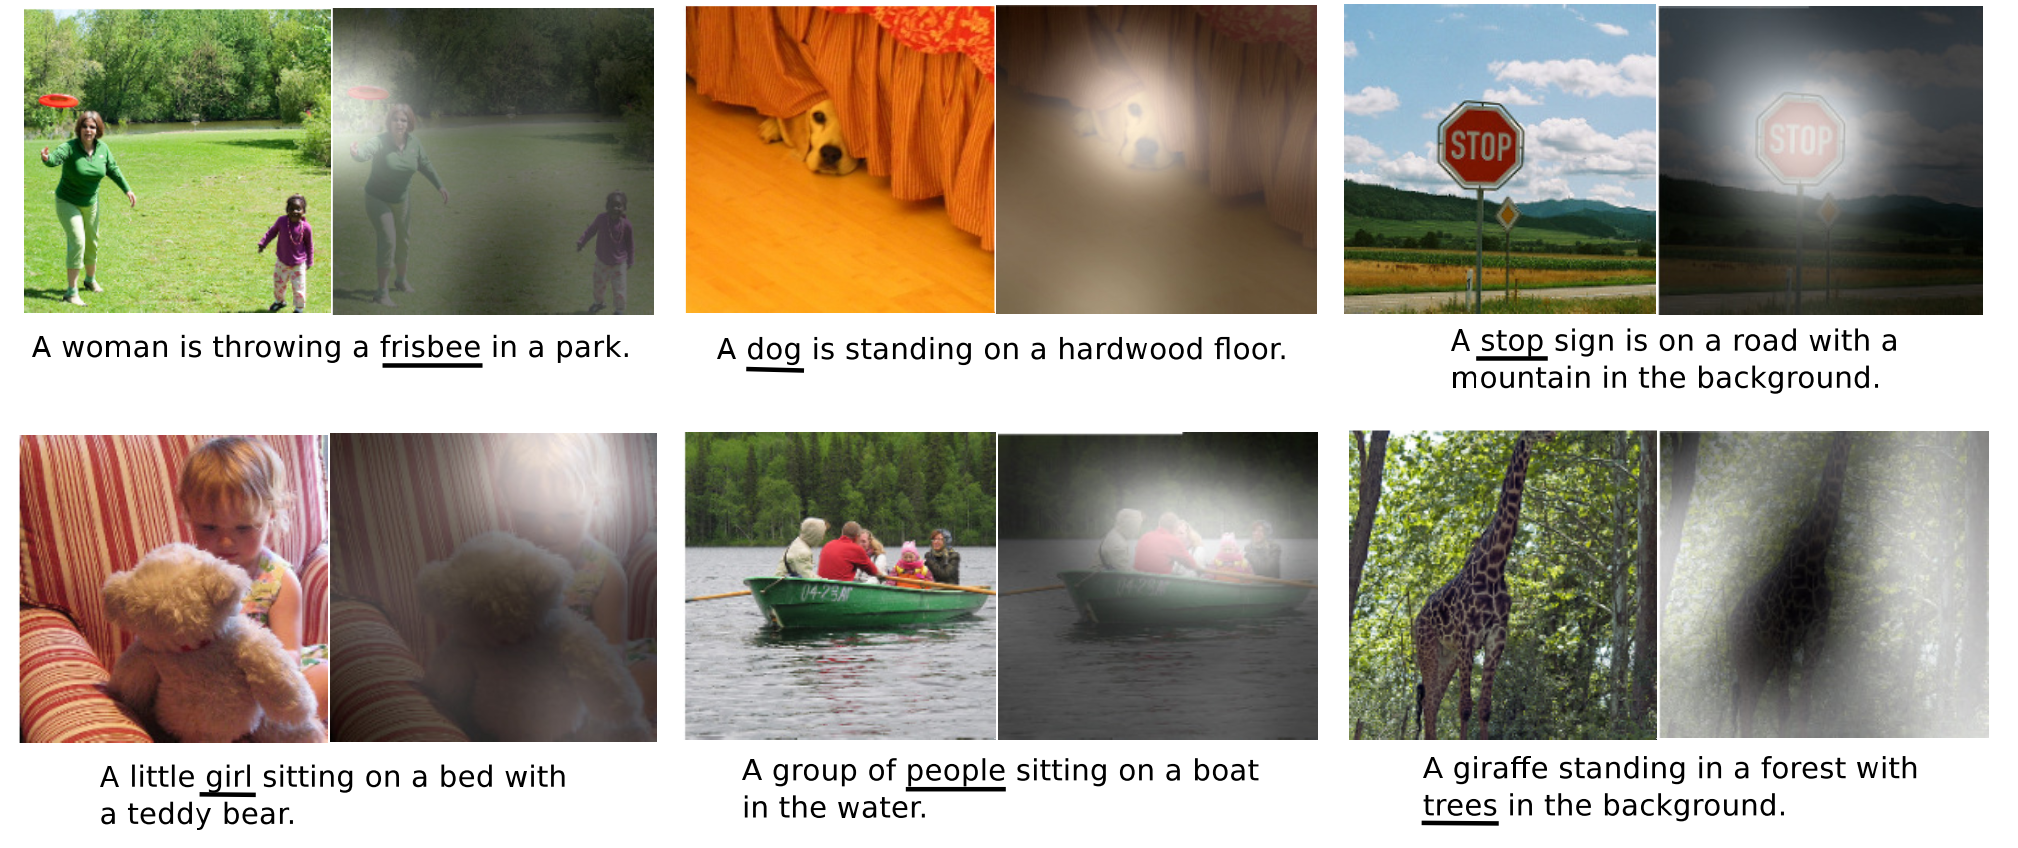
\includegraphics[width=\textwidth]{images/xucaption}
\caption{Attention of a caption generating neural model \citep{xu2015captioning}. The model learns to highlight the correct object when generating words.}
\label{fig:caption}
\end{figure}


While successful, existing seq2seq methods are limited by the length of source and target sequences. For a problem such as document summarization, the source sequence of length $N$ requires $O(N)$ model computations to encode, where $N$ could potentially be very large. However, it makes sense intuitively that not every word of the document will be necessary for generating a summary, and so we would like to reduce the amount of necessary computations over the source document.

Therefore, in order to scale seq2seq methods for this problem, we aim to prune down the length of the source sequence in an intelligent way. The natural solution is to force the model to only use a subset of the input rather than naively encoding the entire input. We investigate some related work in this area.


\section{Conditional Computation}


%The problem of full document summarization, however, is still very open. In order to make the models work, \cite{nallapati2016seq2seq} use a variety of tricks: limiting the decoder vocabulary to the document, the use of pointer attention for \texttt{<unk>} tokens, etc. Our goal in this paper is not necessarily to optimize performance, but to understand how to scale up existing seq2seq methods in an efficient way, and so we attempt to eliminate the use of these ad-hoc tricks whenever possible. We aim to find the best implementation of ``hard'' attention, in which a discrete subset of the source document is selected at any given time, to satisfy the scalability condition.


Many techniques have been proposed in the literature to handle the problem of large inputs to deep neural networks.

The term ``conditional computation'' was coined by \citet{BengioLC13}, where the idea is to compute a subset of units for a given network per input. This would have the advantage of being highly efficient, especially for networks that handle extremely large inputs as is common in vision and NLP.


Conditional computation in practice is usually implemented through the use of discrete units --- these can serve as gates to select certain parts of the network for computation.

\todo{needs some reorganizing}

Unfortunately, discrete variables cannot be backpropagated through as they are either not differentiable or produce zero gradient. Several techniques have been proposed to get around this problem.

\citet{BengioLC13} propose the \emph{straight-through} estimator for binary stochastic gates. We simply sample from the stochastic gates in the forward step, and backpropagate the gradient as if we had not sampled. While this works empirically for simple binary gates, it is theoretically unjustified.


In general, we may want to sample from multinomial distributions, i.e. select one choice out of multiple choices. In deep networks, the softmax function $\operatorname{softmax} : \reals^m \to [0,1]^m$ is used to produce a normalized probability distribution out of any vector of reals. For $\boldz \in \reals^m$,
\begin{equation}
\operatorname{softmax}(\boldz)_i = \frac{\exp(z_i)}{\sum_j \exp(z_j)}
\end{equation}

\citet{rae2016sparsememory} use an approximate nearest neighbors approach for their ``sparse access memory'' model to train a large-scale neural Turing machine. \citet{Shazeer2017} introduce a mixture-of-experts model that selectively chooses a subset of ``expert'' networks at any given time during training. In the spirit of conditional computation, they only train $K$ experts at a time using a sparse gating function.

\citet{martins2016sparsemax} propose an alternative to softmax called the \emph{sparsemax} function. For a given $\boldz$, sparsemax projects the point to the probability simplex. It turns out that this function has a useful gradient while having a sparse output. The downside is that we are not guaranteed to have a one-hot vector as we get from sampling the multinomial distribution.



%\citet{Maddison2017} apply a smoothed version of the Gumbel max trick in order to approximate the sampling process. The Gumbel max trick is an alternative method for sampling multinomial random variables: by drawing i.i.d. uniform variables $U_i \sim \mathrm{Unif}(0,1)$, taking the argmax of $z_i - \log(-\log(U_i))$ gives us a sample with the correct probability. While this process is still discrete and has no gradient, \citet{Maddison2017} use a softmax instead of a max to obtain a smooth approximation that can be differentiated.


Reinforcement learning has also been proposed as an approach to handling discrete units in a network.
\citet{xu2015captioning} suggest ``hard'' attention as one possible discrete selection mechanism. While standard ``soft'' attention averages the representations of where the model attends to, for hard attention we make a hard decision and choose only one location. To train such models, we can use reinforcement learning.

In the next section, we briefly overview reinforcement learning and explain how it can be applied to train the hard attention model.


\section{Reinforcement Learning}

Standard backpropagation training of neural networks assumes that the output is a deterministic and differentiable function of the input. Reinforcement learning, however, is a more general framework that makes no such assumptions.

The traditional setup of reinforcement learning (RL) assumes some agent is navigating an environment and earning rewards.
We assume a state space $\mcS$, an action space $\mcA$, a reward function of state and action $R : \mcS \times \mcA \to \reals$, and a Markovian transition distribution $p(s' | s, a)$ for $s, s' \in \mcS$ and $a \in \mcA$.

We suppose that at time $t$, the agent is in state $s_t \in \mcS$, makes an action $a_t \in \mcA$, earns a reward $r_t = R(s_t, a_t)$, and transitions probabilistically to the next state $s_{t+1}$.
Assuming the reward function is unknown, the agent wants to maximize total expected reward
$$\mathbb{E}_{s_t, r_t} [\sum_{t=0}^\infty \gamma^t r_t]$$
by finding an optimal action policy, i.e. finding the optimal policy $\pi : \mcS \to \mcA$ for states $s \in \mcS$. Here, $\gamma$ is a time discount factor for the reward.


In general RL, we assume that we don't know the reward function $R(s,a)$ and we don't know the transition distribution $p(s_{t+1} | s_t, a_t)$. While the environment still gives us rewards for actions, finding the optimal policy requires predicting which states lead to those rewards.
Since we don't know ahead of time which states are best, we must explore the state space to find what actions lead to the best rewards.

There are several methods for solving the general RL problem. Some are model-based, which attempt to model the transition distribution $p(s_{t+1} | s_t, a_t)$; others are model-free, which directly attempt to learn actions based on states. One such is Q-learning \citep{Watkins1989}, which estimates the reward for every pair $(s,a) \in \mcS \times \mcA$.

Another method is to learn a direct policy function $\pi( \cdot ; \theta) : \mcS \to \mcA$, where $\pi$ is parametrized by weights $\theta$. We can train $\pi$  to maximize expected reward through a gradient ascent method known as \emph{policy gradient}, or the REINFORCE algorithm \citep{williams1992reinforce}.

It turns out that REINFORCE can be used to train deep neural networks with stochastic units by a simple extension of the backpropagation algorithm. In the next section, we derive the training algorithm.

%When the transition distribution $p(s_{t+1} | s_t, a_t)$ and reward function $R(s,a)$ is known, our problem is also known as a Markov decision process (MDP), and can be 
%
%. We can compute an optimal value function $Q(s, a)$ that represents the estimated reward from taking action $a$ in state $s$:
%\begin{align}
%Q(s, a) & = R(s, a) + \gamma \sum_{s' \in \mcS} p(s' | s, a) V(s') \\
%V(s) &= \max_{a \in \mcA} Q(s,a)
%\end{align}
%for every $s \in \mcS, a \in \mcA$. These equations are known as the Bellman equations, and finding an optimal policy then amounts to solving this system for $\pi$. This can be done by treating the system as a fixed point problem and using iterative methods. % citation
%
%When we don't know the transition distribution, we can estimate it by standard maximum-likelihood methods and exploration of the state space. The same iteration techniques then apply.



%There are two methods for approaching the general RL problem. First, model-based approaches attempt to estimate the transition distribution $p(s_{t+1} | s_t, a_t)$ and apply the Bellman equations to find the optimal policy. Second, model-free approaches forgo the transitions and simply learn what action is best in a given state.

%\subsection{Model-free approaches}
%
%We consider the model-free approach in more detail.
%
%\paragraph{Q-learning} One technique is to model the Q-function $Q(s,a)$ that estimates the total reward of action $a$ in state $s$. To learn the Q-function, we predefine some policy based on our current estimates of the Q-function, and we make learning updates as
%\begin{equation}
%Q(s,a) \gets Q(s,a) + \eta \left(r + \gamma \max_{a' \in \mcA} Q(s', a') - Q(s,a) \right)
%\end{equation}
%upon taking action $a$ in state $s$, where $\eta$ is a learning rate, $r$ is the reward received, and $s'$ is the state we transition into. This is known as the \emph{Q-learning} update rule. An alternative update rule takes into account the action $a'$ we would take next in state $s'$:
%\begin{equation}
%Q(s,a) \gets Q(s,a) + \eta  \left(r + \gamma Q(s', a') - Q(s,a) \right)
%\end{equation}
%This is known as the SARSA update rule.
%
%In both cases, if we have a large state space, we may not want to record $Q(s,a)$ for every pair of $s,a$. We can instead parametrize $Q(s,a)$ with weights $w$, and maximizing reward using backpropagation gives us the update rule
%\begin{equation}
%\label{eq:reinforce}
%w \gets w + \eta \left(r + \gamma \max_{a' \in \mcA} Q(s', a') - Q(s,a) \right) \frac{\partial Q(s,a)}{\partial w}
%\end{equation}



%\paragraph{TD-learning} An alternative to modeling the Q-function is to model the value function $V(s) = \max_{a \in \mcA Q(s,a)$, which can be a simpler learning problem. 
%
%Again, suppose we parametrize $V(s)$ with weights $w$, and suppose we have an observed sequence of states $s_t$ and rewards $r_t$. Instead of making updates to $V(s)$ independently for each time $t$, we can take into account our entire trajectory, giving the update rule at time $t$
%\begin{equation}
%w \gets w + \eta \left(r_t + \gamma V(s_{t+1}) - V(s_t) \right) \sum_{k=1}^t \lambda^{t-k} \frac{\partial V(s_k)}{\partial w}
%\end{equation}
%where $\lambda$ is a discount factor for past gradients.
%
%This update is known as the $TD(\lambda)$ update, and is a special case of temporal difference learning (or TD-learning). Taking into account the entire trajectory allows us to obtain more information about which past actions and states led to the best rewards. TD-learning was used to train a world-class backgammon bot \citep{Tesauro1994}.

%This raises two problems. First is the \textbf{credit assignment problem}: we don't know which actions we chose in the past led us to the best rewards. For example, if we are one move away from winning a game and earning a big reward, we don't assign the credit of the reward to that one move, but rather to some good moves we made in the past that led us to the winning state.
%Second is the \textbf{exploration-exploitation problem}. On one hand, we need to explore the state space to determine which states have the best rewards, but on the other hand, we are missing the opportunity to exploit the known high-reward actions.

%occasionally choosing random actions to better explore the state space (also known as an $\epsilon$-greedy exploration policy).


\section{Stochastic Computation Graphs}

Neural networks with stochastic units are also known as \emph{stochastic computation graphs}, as defined by \citet{schulman2015backprop}. Formally, they define a stochastic computation graph (SCG) as a directed, acylic graph with three kinds of nodes:
\begin{enumerate}
\item Input nodes, including fixed network inputs and parameters.
\item Deterministic nodes, which are deterministic functions of their parents.
\item Stochastic nodes, which are random variables distributed conditionally on their parents.
\end{enumerate}
We can formulate a training problem for SCGs by choosing certain terminal nodes and taking their sum as the objective function. If a node is stochastic, we take its expectation. That is, for a set of terminal nodes $\mcC$, we optimize $\sum_{c \in \mcC} \mathbb{E}[\hat{c}]$, where $\hat{c}$ denotes the random variable corresponding to node $c$.

Note that the SCG formulation captures both supervised deep learning and RL policy functions. Deep neural networks are just SCGs with all deterministic nodes, and the loss function $\mcL$ of the task is the objective. The RL policy function is an SCG with actions at the stochastic nodes, and the expected reward $\mathbb{E}[r]$ is the objective. As we will see, SCGs will turn out to be a generalization of the REINFORCE algorithm.

\begin{figure}
% todo
\caption{Simple examples of stochastic computation graphs (SCGs). Nodes in circles are stochastic, nodes in squares are deterministic, and the rest are input nodes. Image from \citet{schulman2015backprop}.}
\label{fig:scg}
\end{figure}

Figure~\ref{fig:scg} shows examples of simple SCGs, as well as the gradient of the objective for the parameter $\theta$. Using the gradient, we optimize the objective function using gradient descent.

Next, we derive the gradient of the objective with respect to parameter input nodes in the general case.

We define for nodes $w,v$ the relation $w \prec v$ (pronounced $w$ influences $v$) if there exists a path from $w$ to $v$ in the SCG. We also say $w \prec^D v$ ($w$ deterministically influences $v$) if there exists a path that consists of only deterministic nodes.

Given an SCG, let $\mcS$ be the set of stochastic nodes, $\mcC$ the set of cost nodes that give the objective. For a given node $v$, let $\on{par}(v)$ denote its parents.

For a given parameter $\theta$, we have the following:
\begin{theorem}
Assume differentiability of all functions. Then the gradient of the objective with respect to $\theta$ is
\begin{align}
\frac{\partial}{\partial \theta} \mathbb{E}\left[ \sum_{c \in \mcC} \hat{c} \right] &= \mathbb{E}\left[\sum_{c \in \mcC} \hat{c} \sum_{v \in \mcS,~\theta \prec^D v, ~v \prec c }  \frac{\partial}{\partial\theta} \log p(v | \on{par}(v) ; \theta )  +
 \sum_{c\in \mcC,~\theta \prec^D c} \frac{\partial}{\partial \theta} \hat{c}
\right] \label{eq:gradient1} \\
&=  \mathbb{E}\left[ \sum_{v \in \mcS,~\theta \prec^D v} \left( \frac{\partial}{\partial\theta} \log p(v | \on{par}(v) ; \theta ) \right) \hat{C}_v + \sum_{c\in \mcC,~\theta \prec^D c} \frac{\partial}{\partial \theta} \hat{c} \label{eq:gradient2}
\right] 
\end{align}
where $\hat{C}_v = \sum_{c \in \mcC, ~v \prec c} \hat{c}$ is a random variable of the cost that stochastic node $v$ influences.
\label{thm:gradient}
\end{theorem}
Before we give the proof, we note the intuition. The first term represents the gradient from the stochastic nodes, where we multiply the gradient of the log probability with the cost.
The second term is the standard gradient we obtain from backpropagation.
\begin{proof}
Due to linearity of expectation, we only need consider a single node $c \in \mcC$. Let $\mcL = \mathbb{E}[\hat{c}]$ be the loss function.

We have stochastic nodes $v$ such that $\theta \prec^D v$ and $v \prec c$. Let this set be $\mcS_\theta$, and denote the joint random variable of this set as $\hat{\boldv}$. Let $c(\hat{\boldv} ; \theta)$ explicitly denote $\hat{c}$.

We compute the gradient:
\begin{align*}
\frac{\partial }{\partial \theta}\mathbb{E}[c] &= \frac{\partial}{\partial \theta} \sum_{\hat{\boldv}} p(\hat{\boldv} | \on{par}(\boldv); \theta) \cdot c(\hat{\boldv}; \theta) \\
& = \sum_{\hat{\boldv}} \frac{ \partial  p(\hat{\boldv} | \on{par}(\boldv); \theta) } {\partial \theta} \cdot c(\hat{\boldv} ; \theta) + p(\hat{\boldv} | \on{par}(\boldv); \theta) \cdot \frac{\partial}{\partial\theta} c(\hat{\boldv}; \theta) \\
&= \sum_{\hat{\boldv}} \frac{ \partial  p(\hat{\boldv} | \on{par}(\boldv); \theta) } {\partial \theta} \cdot c(\hat{\boldv} ; \theta) + \mathbb{E}_{\boldv}\left[ \frac{\partial}{\partial\theta} c(\hat{\boldv}; \theta)  \right]
\end{align*}
Note that the second term gives the standard backpropagation gradient. We can rewrite the first term:
\begin{align*}
\sum_{\hat{\boldv}} \frac{ \partial  p(\hat{\boldv} | \on{par}(\boldv); \theta) } {\partial \theta} \cdot c(\hat{\boldv} ; \theta)
&= \sum_{\hat{\boldv}} p(\hat{\boldv} | \on{par}(\boldv); \theta) \frac{1}{p(\hat{\boldv}|\on{par}(\boldv);\theta)}\frac{ \partial  p(\hat{\boldv} | \on{par}(\boldv); \theta) } {\partial \theta} \cdot c(\hat{\boldv}; \theta) \\
&= \sum_{\hat{\boldv}} p(\hat{\boldv} | \on{par}(\boldv); \theta) \frac{ \partial  \log p(\hat{\boldv} | \on{par}(\boldv); \theta) } {\partial \theta} \cdot c(\hat{\boldv}; \theta) \\
 &= \mathbb{E}_{\hat{\boldv} \sim p(\hat{\boldv} | \on{par}(\boldv); \theta)} \left[ \frac{ \partial  \log p(\hat{\boldv} | \on{par}(\boldv); \theta) } {\partial \theta} \cdot c(\hat{\boldv} ; \theta) \right] \\
&= \mathbb{E}\left[ \widehat{c} \cdot \sum_{v \in \mcS_\theta} \frac{  \partial  \log p(\hat{v} | \on{par}(v); \theta) } {\partial \theta}  \right]
\end{align*}
where the last equality follows from separating the log joint probability term into its conditional marginals.

We have thus shown Equation~\ref{eq:gradient1}. Equation~\ref{eq:gradient2} follows directly by rearranging the order of summations, noting which nodes $v$ influence a certain $c$.

\end{proof}

Because the expectation in both gradient formulae are intractable in the general case, we use a single Monte Carlo sample.
In practice, however, the variance of the Monte Carlo gradient can be very high.

%The training problem can be formalized as an RL problem. We can treat a neural network as a stochastic agent, and its computation serves to define the parametrized policy function $\pi(\cdot; w) : \mcS \to \mcA$.
%The states $\mcS$ are the inputs and the actions $\mcA$ are the possible outputs of each stochastic unit. The rewards are then negative loss (e.g. from regression or classification).


One of the simplest ways to reduce the variance of the gradient estimator is to introduce a baseline scalar $b \approx \mathbb{E}[\hat{c}]$ which we subtract from each cost term. That is, we have:
\begin{theorem}
The gradient from Theorem~\ref{thm:gradient} can also be written as
\begin{equation}
\frac{\partial}{\partial \theta} \mathbb{E}\left[ \sum_{c \in \mcC} \hat{c} \right] = \mathbb{E}\left[\sum_{c \in \mcC} (\hat{c} - b_c) \sum_{v \in \mcS,~\theta \prec^D v, ~v \prec c }  \frac{\partial}{\partial\theta} \log p(v | \on{par}(v) ; \theta )  +
 \sum_{c\in \mcC,~\theta \prec^D c} \frac{\partial}{\partial \theta} \hat{c}
\right] 
\end{equation}
where $b_c$ is a scalar not influenced by any of the $v$ in the summation.
\end{theorem}

\begin{proof}
The proof boils down to a trick with the log probability. Considering a single $c$, by linearity it suffices to show that
\begin{equation*}
\mathbb{E} \left[ \frac{\partial}{\partial\theta} \log p(v | \on{par}(v) ; \theta) \right] = 0, \qquad \forall v \in \mcS_\theta
\end{equation*}
This is true since the $b_c$ term is constant with respect to the expectation (by our assumption that no $v$ influences it).

But this follows since
\begin{align*}
\mathbb{E} \left[ \frac{\partial}{\partial \theta} \log p(\hat{v} | \on{par}(v); \theta) \right] &= \sum_{\hat{v}} p(\hat{v} | \on{par}(v); \theta) \frac{\partial \log p(\hat{v} | \on{par}(v); \theta)}{\partial \theta} \\
&=  \sum_{\hat{v}} p(\hat{v} | \on{par}(v); \theta) \frac{1}{p(\hat{v} | \on{par}(v); \theta)} \frac{\partial  p(\hat{v} | \on{par}(v); \theta)}{\partial \theta}  \\
&= \frac{\partial}{\partial \theta} \sum_{\hat{v}} p(\hat{v} | \on{par}(v); \theta) =  \frac{\partial}{\partial \theta} [1] = 0
\end{align*}
Thus, the gradient with baseline is unbiased.
\end{proof}

Including a baseline is proven to reduce the variance of the estimator \citep{Weaver2001}. There are several different methods for producing baselines, and we will not cover all of them here.

\subsection{Algorithm}
\label{sec:algorithm}

In order to compute the gradients of SCGs in practice, we make a slight tweak to the backpropagation algorithm.

We first perform a forward pass of the SCG to obtain all values and samples for each node. In the backward pass, gradients for nodes that are directly connected to the cost nodes can be computed with usual backpropagation. For stochastic nodes, we first compute the costs $\hat{C}_v$ for node $v$ in Equation~\ref{eq:gradient2}. Broadcasting these values to the corresponding nodes, we can then continue backpropagation from the stochastic nodes with the gradient of the log probability.

Finally, if $g_\theta$ is the resulting gradient for parameter $\theta$, our gradient descent update is
\begin{equation}
\theta \gets \theta  - \eta g_\theta
\end{equation}
where $\eta$ is a learning rate.

Algorithm~\ref{alg:reinforce} gives the complete algorithm for gradient descent on SCGs.



\begin{algorithm}
\caption{Gradient Descent for SCGs}
\label{alg:reinforce}
\begin{algorithmic}
\State Forward pass through SCG
\ForAll{$c \in \mcC$}
\State $\hat{c} \gets \hat{c} - b_c$ \Comment{Subtract baselines from costs}
\EndFor
\ForAll{$v \in \text{SCG}$}
\State $\boldg_v = \begin{cases} 1 & \text{if $v \in \mcC$} \\ 0 & \text{else} \end{cases}$
\State Compute $\hat{C}_v \gets \sum_{c \in \mcC, ~v \prec c} \hat{c}$ \Comment{Aggregated costs}
\EndFor

\For{$v$ in \textsc{ReverseTopologicalOrder}(SCG)}
\For{$w \in \on{par}(v)$}
\If{\textbf{not} \textsc{IsStochastic}($w$)}
\If{\textsc{IsStochastic}($v$)}
	\State $\boldg_w \text{ += } \hat{C}_w \cdot \frac{\partial}{\partial w} \log p(v | \on{par}(v) ) $
\Else
	\State $\boldg_w \text{ += } (\frac{\partial v}{\partial w})^\top \boldg_v$
\EndIf
\EndIf
\EndFor
\EndFor
\ForAll{parameters $\theta$}
\State $\theta \gets \theta - \eta g_\theta$ \Comment{Gradient descent}
\EndFor
\end{algorithmic}
\end{algorithm}


%Our policy gradient update from equation~\ref{eq:reinforce1} can therefore be summarized as
%\begin{equation}
%w^{(t+1)} \gets w^{(t)} + \eta \mathbb{E}_{a_t} \left[ (R_t - b) \frac{\partial \log p(a_t | s_t; w)}{\partial w} \right]
%\end{equation}

While SCGs are a very useful and general framework, it is often simpler to pose certain SCGs in the language of reinforcement learning.

Consider in particular the sequential decision problem of RL. Suppose we have a trajectory of states $s_t$ and we make actions $a_t$ at time $t$ based on some parameterized policy function. Each action leads to a reward $r_t$, and influences total future reward $\sum_{s=t}^T r_s$ where $T < \infty$ is the time horizon.

Note that we can treat our actions $a_t$ for $ t = 0, \ldots, T$ as stochastic nodes in an SCG, and the costs $\hat{c}$ are the rewards we receive for each $t$. Then instead of computing $\hat{C}_{a_t} = \sum_{s=t}^T r_s$, we can scale later rewards with a discount factor $\gamma $, giving
\begin{equation}
\hat{C}_{a_t} = \sum_{s=t}^T \gamma^{s-t} r_s
\end{equation}
which fits neatly in with Algorithm~\ref{alg:reinforce}. We will use this RL setup to discuss our models, and our algorithms are confidently backed up by the theory of SCGs.

\todo{diagram?}




\section{Reinforcement Learning in NLP}
\todo{needs some organizing}

Even before the concept of SCGs were formalized, reinforcement learning and deep learning have successfully been combined to play Go \citep{Silver2016}, 
control robots \citep{Levine2016}, and play Atari games from pixels \citep{deepatari2015}.
In computer vision, policy gradient methods have been fairly successful on several tasks
\citep{mnih2014visualattention, ba2015visualattention, xu2015captioning}.

In NLP, reinforcement learning research is still preliminary, but has been attempted with varying degrees of success so far.
\citet{ranzato2015} apply RL to improve sequential estimation by e.g. training on BLEU rewards for machine translation.
\citet{Narasimhan2015} use RL play text-based games.
\citet{li2016dialogueRL} use RL to train an end-to-end dialogue system.
\citet{narasimhan2016} use RL to improve information extraction on scarce data.
%\citet{Andreas2016} uses RL to compose 
\citet{Yogatama2017} use RL along with an architecture called a tree LSTM that produces a tree-structured latent variable on a sentence using \textsc{Shift} and \textsc{Reduce} actions. They show that the tree LSTM can produce reasonable parse structures by solely using RL methods.


Inspired by these recent works, we are interested to see if reinforcement learning can be applied to the document summarization problem. We will introduce stochastic nodes into a deep learning model and investigate the feasibility of using policy gradient methods for conditional computation.

In the next chapter we describe our models in detail.


\chapter{Models}
\label{chap:models}


\todo{lots of figures needed}

\section{Sequence-to-sequence (seq2seq)}

We first describe the neural network architecture of the seq2seq models, also known as encoder-decoder models \citep{bahdanau2014neural}.


In the seq2seq model, an \emph{encoder} recurrent neural network (RNN) reads the source sequence as input to produce the \emph{context}, and a \emph{decoder} RNN generates the output sequence using the context as input.  One popular RNN choice is the long-short term memory (LSTM) network \citep{hochreiter1997long}.


More formally, suppose we have a vocabulary $\mcV$. A given input sentence $w_1, \ldots, w_n \in \mathcal{V}$ is transformed into a sequence of vectors $\boldx_1, \ldots, \boldx_n \in \mathbb{R}^{d_{in}}$ through a word embedding matrix $\boldE \in \mathbb{R}^{|\mathcal{V}| \times d_{in}}$ as $\boldx_t = \boldE w_t$.

An RNN is given by a parametrizable function $f_{enc}$ and a hidden state $\boldh_t \in \mathbb{R}^{ d_{hid}}$ at each time step $t$ with $\boldh_t = f_{enc}(\boldx_t, \boldh_{t-1})$. For the LSTM, we keep an auxiliary state $\boldc_t$ along with $\boldh_t$, and we compute $f_{enc}$ as
\begin{align}
\boldf_t &= \sigma(\boldW^f \boldx_t + \boldU^f \boldh_t + b_f) \\
\boldi_t &= \sigma(\boldW^i \boldx_t + \boldU^i \boldh_t + b_i) \\
\boldo_t &= \sigma(\boldW^o \boldx_t + \boldU^o \boldh_t + b_o) \\
\boldc_t &= \boldf_t \odot \boldc_{t-1}  + \boldi_t \odot \tanh(\boldW^c \boldx_t + \boldU^c \boldh_{t-1} + b_c) \\
\boldh_t &= \boldo_t \odot \tanh(\boldc_t)
\end{align}
where $\boldW, \boldU, b$ are learned parameters, and $\odot$ is the elementwise product. 
Intuitively, $\boldc_t$ is the memory cell, $\boldf_t$ is the forget gate, $\boldi_t$ is the input gate, $\boldh_t$ is the output cell, and $\boldo_t$ is the output gate.

LSTMs can be stacked on top of one another by treating the outputs $\boldh_t$ of one LSTM as the inputs to another LSTM.

In stacked LSTMs, we will take the top sequence of hidden states $\boldh_1, \ldots, \boldh_n$ to form a single context vector.


The decoder is another RNN $f_{dec}$ that generates output words $y_t \in \mathcal{V}$. It keeps hidden state $\boldh_t^{dec} \in \mathbb{R}^{d_{hid}}$ as $\boldh_t^{dec} = f_{dec}(y_{t-1}, \boldh_{t-1}^{dec})$ similar to the encoder RNN.
A context vector is produced at each time step using an attention function $a$ that takes the encoded hidden states $[\boldh_1, \ldots, \boldh_n]$ and the current decoder hidden state $\boldh_t^{dec}$ and produces the context $\boldc_t \in \reals^{d_{ctx}}$:
\begin{equation}
\boldc_t = a([\boldh_1, \ldots, \boldh_n], \boldh_t^{dec})
\end{equation}
As in \citet{luong2015effective}, it is helpful to feed the context vector at time $t-1$ back into the decoder RNN at time $t$, i.e. $\boldh_t^{dec} = f_{dec}([y_{t-1}, \boldc_t], \boldh_{t-1}^{dec})$.

Finally, a linear projection produces a distribution over output words $y_t \in \mcV$:
\begin{equation}
p(y_t | y_{t-1}, \ldots, y_1, [h_1, \ldots, h_n]) = \boldW^{out}\boldc_t + b^{out}
\end{equation}

Given document-summary pairs $\{ (\boldx^{(i)}, \boldy^{(i)}) \}_{i=1}^N$ for training, the models are trained to maximize the log probability of getting the sequences in the dataset correct, i.e. minimize the negative log-likelihood (NLL):
\begin{align*}
\mcL(\theta) &= - \sum_{i=1}^N \log p(\boldy^{(i)} | \boldx^{(i)}; \theta)  \\
&= -\sum_{i=1}^N \sum_{t=1}^{T-1} \log p(y_{t+1}^{(i)} | \boldx^{(i)}, y_t^{(i)}, \ldots, y_1^{(i)} ; \theta)
\end{align*}
As the model is fully differentiable with respect to its parameters, we can train it end-to-end with stochastic gradient descent and the backpropagation algorithm.

We note that we have great flexibility in how our attention function $a$ combines the encoder context and the current decoder hidden state. In the next few sections, we explain standard choices for $a$ as well as our proposed coarse-to-fine attention model.

\section{Model 0: Standard Attention}

In \cite{bahdanau2014neural}, the function $a$ is implemented with an \emph{attention network}. We compute attention weights for each encoder hidden state $h_i$ as follows:
\begin{align}
\beta_{t,i} &= \boldh_i^\top \boldW^{attn} \boldh_t^{dec} \quad \forall i = 1, \ldots, n\\
\balpha_t &= \mathrm{softmax}(\bbeta_t) \\
\widetilde{\boldc}_t &= \sum_{i=1}^n \alpha_{t,i} \boldh_i
\end{align}
The idea behind attention is to select the most relevant words of the source (by assigning higher attention weights) when generating output word $y_t$ at time $t$.

The $\mathrm{softmax}$ function, defined as
\begin{equation}
\mathrm{softmax}([\beta_1, \ldots, \beta_n])_i =  \frac{\exp(\beta_i)}{\sum_{j=1}^n \exp(\beta_j)}
\end{equation}
normalizes the $\alpha_i$ to sum to 1 over the source sentence words. This gives us a notion of probability distribution over the encoder words --- we can therefore write $\boldc_t$ as the expectation $\mathbb{E}_\alpha[\boldh]$, where we pick $\boldh_i$ with probability $\alpha_i$.

Our final context vector is then
\begin{equation}
\boldc_t = \tanh(\boldW^2[\widetilde{\boldc}_t, \boldh_t^{dec}])
\end{equation}
for $\boldW^2 \in \reals^{2d_{hid} \times d_{ctx}}$ a learned matrix.

Going forward, we call this instantiation of the attention function \textsc{Model 0}.


\section{Model 1 and 2: Coarse-to-Fine Soft Attention}

\begin{figure}
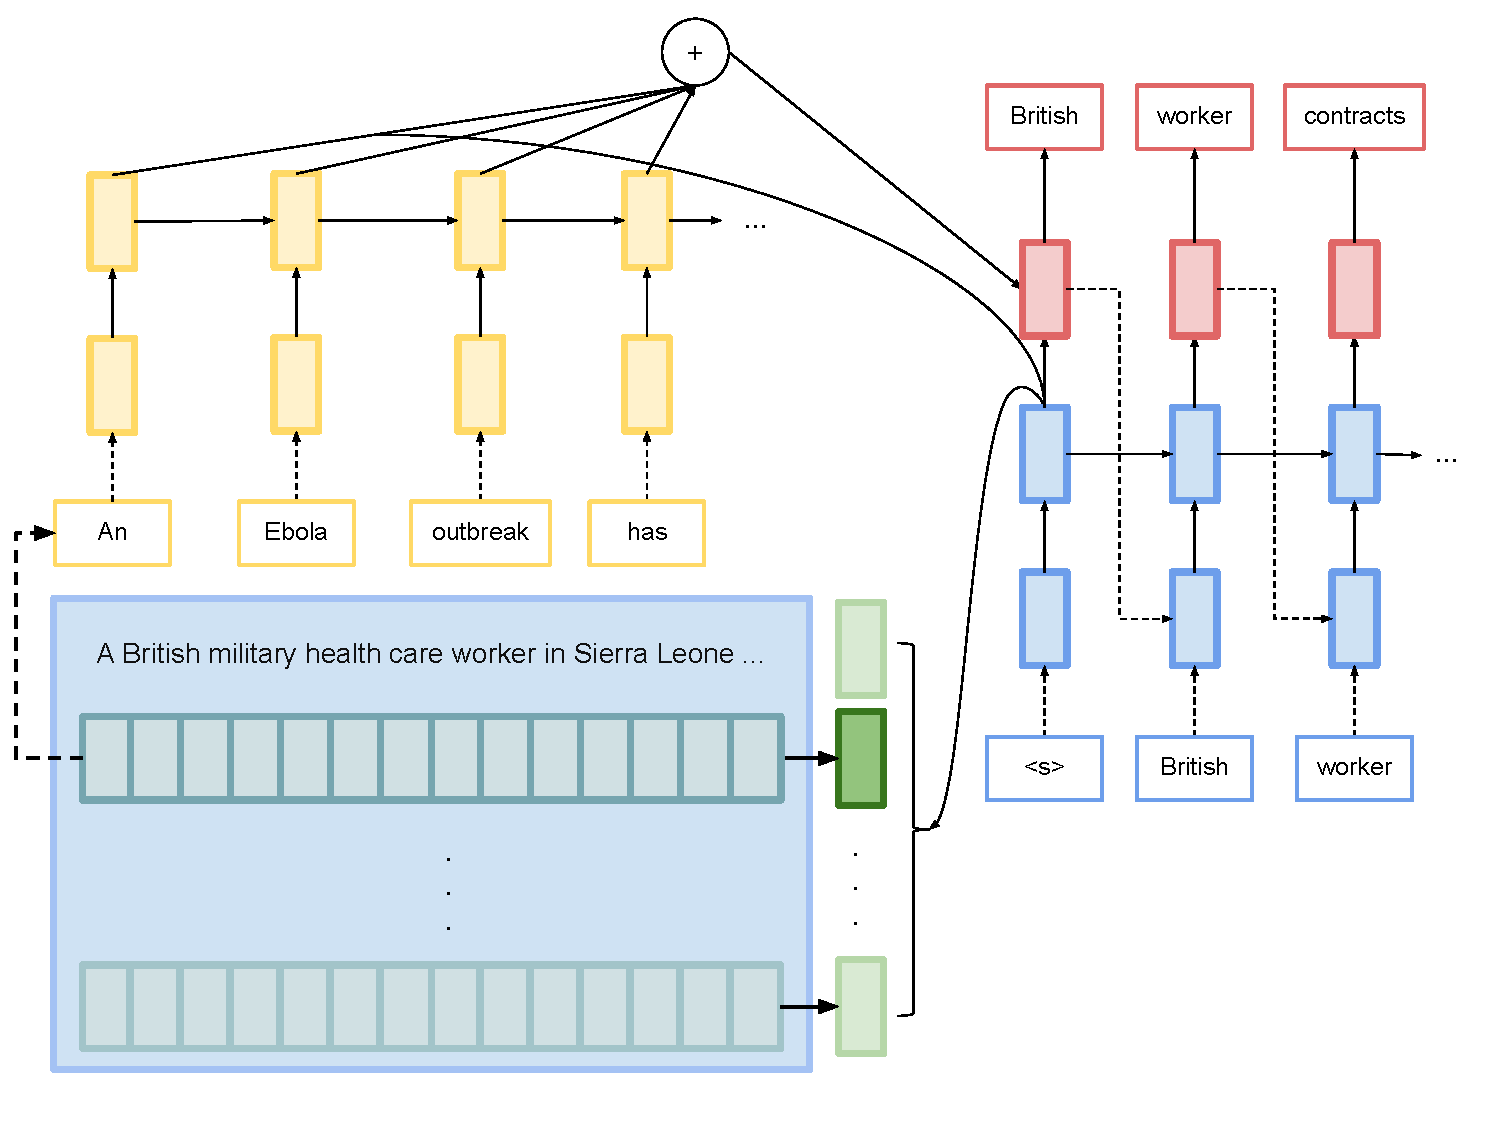
\includegraphics[width=\textwidth]{images/coarse_to_fine.pdf}
\caption{Model architecture for sequence-to-sequence with coarse-to-fine attention. The left side is the encoder that reads the document, and the right side is the decoder that produces the output sequence. On the encoder side, the green hidden states (sentence-level) are used for the coarse attention weights, while the yellow hidden states (word-level) are used for the fine attention weights. The context vector is then produced by averaging the word-level states. In \textsc{Model 2}, we average over the coarse attention weights, thus requiring computation of all word-level hidden states. In \textsc{Model 3}, we make a hard decision for which sentence to use, and so we only need to compute word-level hidden states for one sentence.}
\label{fig:coarsetofine}
\end{figure}

We can leverage the same idea for text summarization, assuming we have a suitable representation of our input document. The simplest method for doing so would be to run an LSTM over the document.

However, the attention step becomes computationally difficult --- for each word we generate, we need to compare it to every word of the document in order to determine which part to attend to. Therefore, we propose a hierarchical method of attending to the document by first attending to sentences, then to the words within sentences. We call this method \emph{coarse-to-fine attention}
\footnote{The term coarse-to-fine attention has previously been introduced in the literature \citep{mei2016}. However, their idea is different: they use coarse attention to reweight the fine attention computed over the entire input. This idea has also been called hierarchical attention \citep{nallapati2016seq2seq}.}.



To be able to attend to both sentences and words in a hierarchical manner, we need to construct encodings of the document at both levels. Thus, we run a low-level LSTM encoder on the words of each sentence for a fine-grained representation of the text, and a simpler encoder model (e.g. bag of words) for coarse-grained sentence representations.
\citet{Sukhbaatar2015} demonstrate how coarse representations can be useful by using memory networks to access information for simple question-answering tasks.
\citet{li2015autoencoder} use the idea of coarse and fine encodings to develop a hierarchical autoencoder for representing paragraphs of text.
%by using low-level LSTMs on words to build sentence representations, then a high-level LSTM on the sentences for the final paragraph representation.

Therefore, if we can make our model first use coarse attention to choose sentences, then use fine attention to choose words only from that sentence, then we avoid the computational cost of searching over the entire document. This idea runs into a very serious problem, however: by posing the attention as a discrete selection process, the neural network loses the key property of being differentiable, and so standard backpropagation no longer applies.

%%%

For a large source input like a document, it may be computationally inefficient to run an RNN over the entire source. Instead, we can consider organizing the document into distinct sentences and select one sentence to attend to at a time.

Specifically, suppose we have sentences $s_1, \ldots, s_m$ with words $w_{i,1}, \ldots, w_{i,n_i}$ for sentence $s_i$, so that we can apply an RNN to each separately to get corresponding hidden states $\boldh_{i,j}$ for $i = 1, \ldots, m$ and $j = 1, \ldots, n_i$.
For attention, we then consider two options.

\paragraph{Model 1} We can follow \textsc{Model 0} and compute attention weights $\alpha_{i,j}$ for each hidden state $\boldh_{i,j}$ by normalizing over all states. We call this \textsc{Model 1}.

\paragraph{Model 2} Alternatively, rather than taking attention over the entire document, we can instead have a two-layered hierarchical attention mechanism: first, we have weights $\alpha_1^s, \ldots, \alpha_m^s$ for each sentence, and then for sentence $s_i$, we have another set of weights $\alpha_{i,1}^w, \ldots, \alpha_{i,n_i}^w$.
Our final attention weight on word $w_{i,j}$ is then $\alpha_{i,j} = \alpha_i^s \cdot \alpha_{i,j}^w$.

In order to compute the sentence attention weights $\alpha_i^s$, we need to produce representations of each sentence; i.e., given the words $w_{i,1}, \ldots, w_{i, n_i}$ of the sentence, we produce a vector representation $\boldh^s_i \in \mathbb{R}^{d_{sent}}$.

\begin{figure}
\caption{Options for producing sentence representations. We can either use a bag of words by summing the word embeddings, or apply convolutions and max-over-time pooling.}
\label{fig:sent_reps}
\end{figure}

Our first option is bag of words: we simply take the representation as
\begin{equation}
\boldh_i^s = \sum_{j=1}^{n_i} \boldE w_{i,j}
\end{equation}
i.e. the sum of the word embeddings, where $\boldE$ is another embedding matrix.

Alternatively, we can use a convolutional method: as in \citet{kim2014convolutional}, we perform a convolution over each window of words in the sentence using a fixed kernel width. We use max-over-time pooling to obtain a fixed-dimensional sentence representation in $\mathbb{R}^{d_f}$ where $d_f$ is the number of filters.

Explicitly, fix a sentence and suppose we have word vectors $\boldx_1, \ldots, \boldx_n$ with $\boldx_j = \boldE w_j \in \reals^{d_{in}}$, and suppose we have kernel width $k$ and convolution weights $\boldW^{conv} \in \reals^{d_f \times d_{in} k}$ where $d_f$ is the number of filters. Then applying the convolution
$\boldW^{conv} * [\boldx_1, \ldots, \boldx_n]$ gives result $\boldu = [\boldu_1, \ldots, \boldu_{n-k+1}]$ with $j$th element
$$\boldu_j = \boldW^{conv} \cdot [\boldx_j, \boldx_{j+1}, \ldots, \boldx_{j+k-1}] + \boldb^{conv} \in \reals^{d_f}$$
Our final output is given by 
\begin{equation}
\boldh^s = \max_j(\tanh(\boldu_j))
\end{equation}
where the max-over-time takes the maximum along the word indexing dimension.


Thus, using the sentence representations, we can compute attention over the sentences.
For the words in each sentence, we run an LSTM over each sentence separately, and create attention weights over each sentence in the same way as \textsc{Model 0}. Using attention on word $w_{i,j}$ as  $\alpha_{i,j} = \alpha_i^s \cdot \alpha_{i,j}^w$, we can proceed exactly as in \textsc{Model 0} by computing the weighted average over hidden states $\boldh_{i,j}$.

We call this method of attention \textsc{Model 2}.

\section{Model 3: Coarse-to-Fine Sparse Attention}

With the previous models, we are required to compute hidden states over all words and sentences in the document, so that if we have $M$ sentences and $N$ words per sentence, the computational complexity is $O(MN)$ for each attention step.

However, if we are able to perform conditional computation and only compute on $M^+$ of the sentences, we can reduce the complexity to $O(M^+N)$. If we are able to make $M^+$ constant or even 1, this would give significant benefits to our overall complexity.

In our experiments, we will apply stochastic sampling to the attention distribution $\balpha$ in the spirit of \citet{xu2015captioning} and ``hard attention''.
Specifically, rather than computing the context $\widetilde{\boldc}$ as an expectation over $\balpha$ (i.e. $\boldc = \sum_{i=1}^n \alpha_i \boldh_i$), we can sample from the probability distribution $\balpha$ to obtain a single state $\boldh_i$, and we set $\widetilde{\boldc} = h_i$ as the sampled hidden state.

In our case, we take \textsc{Model 2} and apply hard attention at the sentence level, but keep the word level attention per sentence as is. That is, we sample from the attention weights $\alpha_1^s, \ldots, \alpha_m^s$ to obtain a one-hot encoding for the sentence attention, and apply the same multiplication with this one-hot vector on the word-level attention weights $\alpha_{i,1}^w, \ldots, \widetilde{\alpha}_{i,n_i}^w$ for all $i = 1, \ldots, m$. We call this \textsc{Model 3}.


Because the hard attention model loses the property of being end-to-end differentiable, we use reinforcement learning to train our network.


\subsection{Practical Considerations}
\label{sec:practical}

Our hard attention model is now a stochastic computation graph, and thus Algorithm~\ref{alg:reinforce} from Section~\ref{sec:algorithm} applies.

Here, we have an RL agent where the state $s_t$ is the LSTM decoder state at time $t$, and actions $a_t$ are the hard attention decisions.
Since samples from $\balpha_t$ at time $t$ of the RNN decoder can also affect future rewards, we use a discount factor of $\gamma = 0.5$, so that the reward is $\hat{C}_t = \sum_{s = t}^n \gamma^{n-s}r_s$ at time $t$, where $r_t = \log p(y_t | y_1, \ldots, y_{t-1}, \boldx)$ is the single step reward.

To calculate the baselines for variance reduction, we store a constant $b_t$ for each decoder time step $t$. We follow \citet{xu2015captioning} and keep an exponentially moving average of the reward for each time step $t$:
\begin{equation}
b_t \gets b_t + \beta (r_t - b_t)
\end{equation}
where $r_t$ is the average minibatch reward and $\beta$ is a learning rate (set to 0.1).

While several papers suggest using a learned baseline \citep[e.g.][]{mnih2014visualattention, ranzato2015}, we have not found this to be effective. In our experiments, we found that attempting to learn the baseline failed to converge, most likely because there is not enough correlation between the reward and the hidden states preceding the attention layer.

In addition to including a baseline, we also scale the rewards by a tuned hyperparameter --- we found that scaling helped to stabilize training. We empirically set this scale to 0.3.



%Similarly, we keep a moving average of the variance for normalization:
%$$\sigma^2_j = (1 - \beta) \sigma^2_{j-1} + \beta v_j$$
%where $v_t$ is the variance of the minibatch rewards for batch $j$. Since we have rewards at each time step of the decoder LSTM, we keep a separate moving average for the baseline for each time step, but we keep a single moving variance for all time steps.




\paragraph{Randomly training using soft attention} \citet{xu2015captioning} explain that training hard attention with REINFORCE has very high variance, even when including a baseline. Thus, for every minibatch of training, they randomly use soft attention instead of hard attention with some probability (they use 0.5).
The backpropagated gradient is then the standard soft attention gradient instead of the REINFORCE gradient.

While this method helps stabilize training, it's aesthetically not very pleasing. Our goal in coarse-to-fine attention is to reduce computation over the encoded hidden states, while this method requires that we perform the full amount of computation as soft attention for a random subset of minibatches. However, we include this training method in our experiments to test how feasible hard attention is.

\section{Beam Search}

At test time decoding, we use beam search. \todo{do we need this?}

%We also include an entropy-increasing term to encourage exploration during the training process, which is important to speed up convergence of learning. Our policy gradient equation then becomes
%\begin{equation}
%w \gets w + (R_t - b) \frac{\partial \log p(\balpha_t | y_1, \ldots, y_{t-1})}{\partial w}
% + \lambda_{ent} \frac{\partial H(\balpha_t)}{\partial \balpha_t}
%\end{equation}
%where $H(\balpha_t) = -\sum_{i=1}^n \alpha_t \log \alpha_t$ is the entropy function and $\lambda_{ent}$ is a hyperparameter.


%\subsection{Multiple Samples}
%
%From our initial experiments with Model 3, we found that taking a single sample was not very effective. However, we discovered that sampling multiple times from the distribution $\alpha$ significantly improves performance.
%
%We sample based on the multinomial distribution $\mathrm{Mult}(k, \{\alpha_i\}_{i=1}^n)$ to produce the sentence-level attention vector $\alpha$ of length $n$, with $\alpha_i = x_i / k$, where $x_i$ is the number of times index $i$ was sampled. $k$ is a hyperparameter which can be tuned, and we found that $k=5$ works well in our experiments.
%
%The intuition here is for the hard attention model to more closely approximate the soft attention model, as it can select more sentences to produce the context.

%\subsection{Curriculum}
%
%Since training using policy gradients tends to be noisy and slow to converge, we experimented with a curriculum that starts training with soft attention and in epoch $t$, trains a minibatch using hard attention with probability $p_t = 1 - 1/\sqrt{t}$ \citep{bengio2016hardntm}.
%
%While we found this to be helpful for single sample hard attention, it was not necessary for effective training with multisampled hard attention. We prefer to train solely with hard attention when possible, as we are able to save computation at training time.

%\section{Sparsemax}
%
%% describe


\chapter{Experiments}
\label{chap:experiments}

\section{Data}

\subsection{CNN/Dailymail}

Experiments were performed on the CNN/Dailymail dataset from \cite{Hermann2015}.
While the dataset was created for a question-answering task, the dataset format is suited for summary. Each data point is a news document accompanied by up to 4 ``highlights'', and we take the first of these as our target summary.



Train, validation, and test splits are provided along with document tokenization and sentence splitting. We do additional preprocessing by replacing all numbers with \# and appending end of sentence tokens to each sentence. We limit our vocabulary size to 50000 most frequent words, replacing the rest with \texttt{<unk>} tokens. We dropped the documents which had an empty source (which came from photo articles).

 Table~\ref{table:data_stats} lists statistics for the CNN/Dailymail dataset. Figure~\ref{fig:data_examples} shows examples source and target pairs from the dataset.



% dataset statistics
\begin{table}[h]
\centering
\begin{tabular}{lccc}
\toprule
Dataset  & CNN & Dailymail & Combined\\
\midrule
Train size & 90266 & 196961 & 287227\\
Valid size & 1220 & 12148 & 13368\\
Test size & 1093 & 10397 & 11490 \\
Avg. \# words per doc. & 794 & 832\\
Avg. \# sent. per doc. & 21 & 29\\
Avg. \# words per sent. & 36 & 27\\
Avg. \# words per summary & 13 & 15 \\
\bottomrule
\end{tabular}
\caption{Statistics for CNN/Dailymail data.}
\label{table:data_stats}
\end{table}

\begin{figure}
\caption{Examples of source and target for the CNN/Dailymail dataset. The source is a news article, and the target is one of the given highlights.}
\label{fig:data_examples}
\end{figure}

In the context of these new datasets, the summarization task has not yet been fully standardized. Research in the area is still largely preliminary, with only a few papers reporting results \citep[][e.g.]{nallapati2016seq2seq}. While CNN/Dailymail may not be the most suitable dataset for the task due to its noisiness \citep{Chen2016}, a better alternative is yet to exist.



%\section{Synthetic Pretraining} % are we still doing this???
%
%We found that unsupervised pretraining on the given dataset is beneficial to learning. For each document, we randomly sample 2 sentences and concatenate to form the target sentence in a new synthetic dataset. We can sample multiple times to have multiple targets for a given source document, and we found that 5 samples was most beneficial to learning (performance drops with significantly more samples). We then train on the synthetic dataset for 5 epochs and initialize future training with the learned weights.

\section{Implementation details}

A few implementation details were necessary to make minibatch training possible. First, instead of taking attention over each individual sentence, we arrange the first 400 words of the document into a 10 by 40 image, and take each row to be a sentence.

Second, we pad short documents to the maximum length with a special padding word, and allow the model to attend to it. However, we zero out word embeddings for the padding states and also zero out their corresponding LSTM states. We found in practice that very little of the attention ended up on the padding words.

Ideally, we would prefer to not truncate documents, especially since later context can be useful for summarizing the document. Due to memory issues, this is a problem we still have to resolve.

\section{Models}

\paragraph{Baselines}
For a baseline, we take the first sentence of the document (chosen as the average length of a sentence in the training dataset). We call this \textsc{First}.

We also consider the feature-based document summarizer of \citet{Durrett2016}, which uses ILP methods to compress extracted sentences. We apply the code \footnote{https://github.com/gregdurrett/berkeley-doc-summarizer} directly on the test set without retraining the system. Their system requires that the documents are preprocessed in CONLL format, and we use the Berkeley coreference system\footnote{https://github.com/gregdurrett/berkeley-entity}.

\paragraph{Our models}

We ran experiments with Models 0 to 3 as described above.

\begin{itemize}
\item Model 0: Soft attention.
\item Model 1: Organized by sentence, soft attention over all.
\item Model 2: Hierarchical LSTM, coarse-to-fine with soft attention.
\item Model 3: Hierarchical LSTM, coarse-to-fine with hard attention over sentences.
%\item Model 3+multisampling: We include multisampling with $k=5$.
\end{itemize}



\section{Training}

%% fix batch size and other details, and also note we train until convergence (which is slightly longer for hard attn)
We train with minibatch stochastic gradient descent (SGD) with batch size 20 for 20 epochs, renormalizing gradients below norm 5. We initialize the learning rate to 0.1 for the sentence encoder and 1 for the rest of the model, and begin decaying it by a factor of 0.5 each epoch after the validation perplexity stops decreasing.\footnote{We tried more complicated SGD optimization methods such as Adagrad \citep{Duchi2011} and Adam \citep{Kingma2015}, but found that they did not perform as well. This could be due to gradient norms that are too large.}

We use 2 layer LSTMs with 500 hidden units, and we initialize word embeddings with 300-dimensional word2vec embeddings \citep{mikolov2013word2vec}. For convolutional layers, we use a kernel width of 6 and 600 filters.

% talk about LSTM soft attention?

%\paragraph{Hard attention}
%Rewards for multisampling are scaled by a factor of $0.04$ (in addition to scaling by the moving variance).



Our models are implemented using Torch \citep{Torch} based on a past version of Harvard's OpenNMT system\footnote{https://github.com/harvardnlp/seq2seq-attn}. We ran our experiments on a GPU (specs?). All of our code is available open source\footnote{https://github.com/jeffreyling/seq2seq-hard}.

In the next chapter we show results.

\chapter{Results}
\label{chap:results}

\section{Evaluation}

We report metrics for perplexity and ROUGE scores \citep{lin2004rouge} on the test set. % will I have time to do the test set??? main problem is running the Berkeley system
ROUGE-n computes n-gram overlap between a gold summary and a predicted summary, and ROUGE-L computes the longest common subsequence.
We use ROUGE balanced F-scores and report numbers for ROUGE-1 (unigrams), ROUGE-2 (bigrams), and ROUGE-L. While ROUGE traditionally uses the recall metric, we choose F-score since recall is biased towards longer predicted sentences.

With multiple gold summaries in the CNN/Dailymail highlights, we choose to take the max ROUGE score over the gold summaries for a predicted summary, as our models are trained to produce a single sentence. The final metric is then the average over all test data points. % check this



\begin{table}[h]
\centering
\begin{tabular}{llcccc}
 \toprule
 Model &  & PPL & ROUGE-1 & ROUGE-2 & ROUGE-L \\
 \midrule
\textsc{First} & & - & 23.1 & 9.8 & 20.5 \\
\textsc{Berkeley} & & - & \\
\textsc{Model 0} & & 13.6 &  \\
 \textsc{Model 1} & & \\
\textsc{Model 2 conv} & & 15.8 & & \\
\textsc{Model 2 sparsemax} & & 16.1 \\
\textsc{Model 3 hard only} & & 32.3 \\
\midrule
\textsc{Model 2 BOW} & & 16.4 & & \\
\textsc{Model 2 LSTM} & & 15.5 \\
\textsc{Model 2 5x80 conv} & & 14.8 \\
\textsc{Model 2 2x200 conv} & & 14.2  \\
\textsc{Model 2 conv +pos} & & 15.3 & & \\
\midrule
\textsc{Model 3 hard sample 2} & & 25.0 \\
\textsc{Model 3 hard sample 3} & &  \\
 \bottomrule
\end{tabular}
\caption{Summarization results for CNN/Dailymail.}
\label{table:summary}
\end{table}

\begin{table}[h]
\centering
\begin{tabular}{llr}
\toprule
Model & & Entropy \\
\midrule
\textsc{Model 0} \\
\textsc{Model 1} \\
\textsc{Model 2 conv} \\
\textsc{Model 2 BOW} \\
\textsc{Model 2 conv +entropy}  \\
\textsc{Model 2 sparsemax} \\
\bottomrule
\end{tabular}
\caption{Entropy over sentence attention. We computed \textsc{Model 0} and \textsc{Model 1} entropy by summing over each row.}
\label{table:entropy}
\end{table}

\section{Analysis}

\todo{fill in numbers, plot training curves, attention heatmaps, predicted summaries}

See Table~\ref{table:summary} for summary results.

We investigate the entropy of the sentence attention on the validation set in Table~\ref{table:entropy}.

% synthetic data

% MT?

% training curves
We see hard attention takes longer to converge.

%% attention figures 
We see that the attention is very spread out over sentences. In particular, we notice that the word-level attention focuses on specific stop words for all decoder time steps. We posit this may be due to ???
See Appendix~\ref{appendix:attn} for more visualizations.

% predicted examples
We show some predicted summaries from the model.

\section{Discussion}

Coarse-to-fine might work but it hurts performance. For next steps, we would want to scale to even larger datasets and implement hard attention.

\chapter{Conclusion}
\label{chap:conclusion}


\bibliographystyle{plainnat}
\bibliography{../papers/Mendeley/library}


\begin{appendices}

\chapter{Attention Visualizations}
\label{appendix:attn}
hi

\end{appendices}

\end{document}
